\section*{Method}
In order to compare the performance of an altas-based segmentation versus a machine learning approach, both methods have been applied to the same set of images. Five brain tissues have been segmented: grey and white matter, amygdala, hippocampus, and thalamus. 
The pipeline used as a basis for the algorithms implementation was intended for a machine learning segmentation approach. For the atlas-based segmentation implementation, the training data from the provided pipeline have been used to generate different atlas according to the methods described below. Since the training data are used to be compiled multi-atlas fusion, it will be refer to the atlas as the result of the fusion from the training images. This work includes the comparison of four different multi-atlas segmentation methods versus the provided machine learning approach described in the previous chapter.
The data are composed of an atlas (N = 1), a training subset (N = 20) and a testing subset (N = 10). Each of those data contain a T1-weighted image (T1w), a T2-weighted image (T2w), a ground truth image, and a brain mask used for skull stripping.

\subsection*{MIA pipeline} \label{sec:MIApipeline}
The medical image analysis pipeline consists of five distinct steps: registration, pre-processing, feature extraction, classification and post-processing. It is illustrated in the fig. \ref{fig:pipeline}.

\begin{figure}[h!]
	\centering
	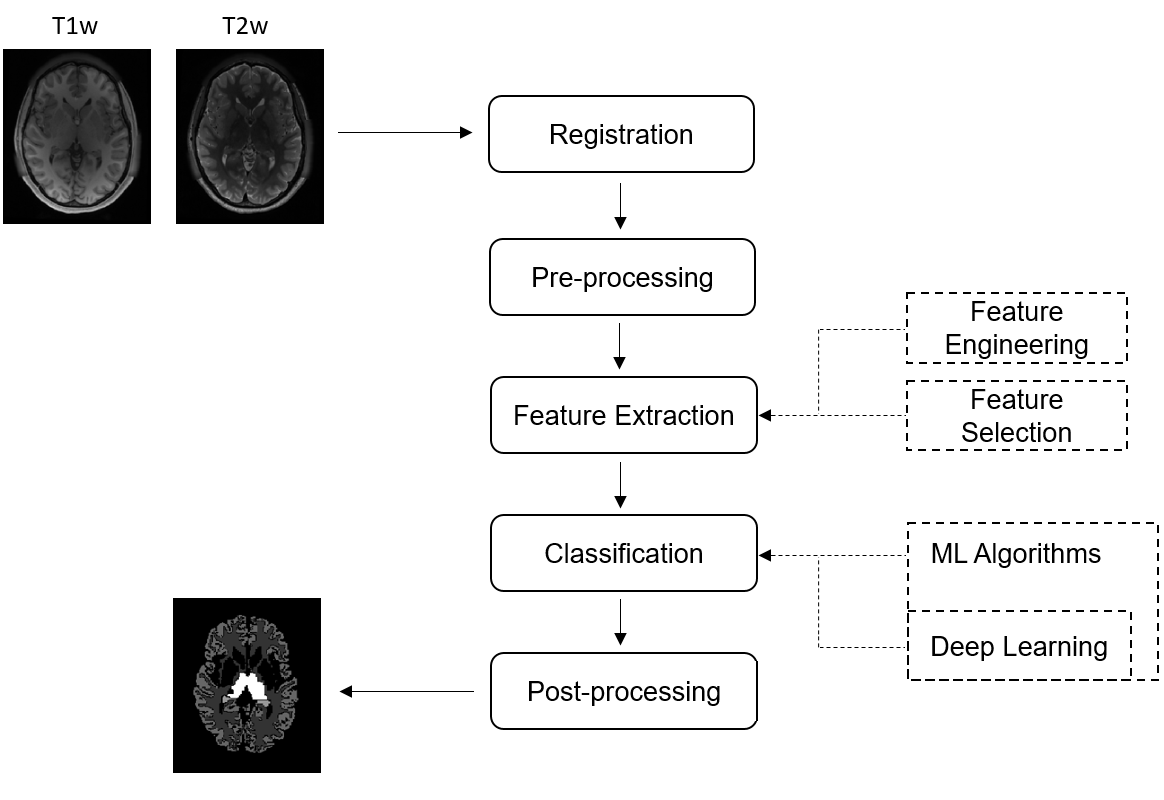
\includegraphics[width = .45 \textwidth]{img/pipeline2}
	\caption{Schematic of the medical image analysis pipeline.}
	\label{fig:pipeline}
\end{figure}

Registration matches an acquired image to a reference one, usually provided from an atlas. This image transformation can be affine as well as non-rigid, which allows local deformations. The pre-processing is used to improve the quality of an image. It uses different kind of filters and masks to get a higher quality image or remove unnecessary data. Intensity normalization is also used, especially if machine learning is involved. Feature extraction tries to find position of anatomical landmarks. Contours and corners can be found with rather simple algorithms. Classification means to decide of the anatomical type for each voxel. This can be done in various ways, decisions trees (also called random forests) in machine learning or by growing regions algorithms. Finally, post-processing gives a cleaner final segmentation. It will remove small groups of voxels that should not correspond to any real anatomical part. As an example, a human body can only have one liver or two kidneys of similar size.

\subsection*{Registration}
For the registration step, two different solutions have been compared. The first is affine transformation, which which allows translation, rotation and scaling. The second one is non-rigid, which transforms the volumes locally. This can lead to a better matching between the input image and the atlas. For the affine registration of two volumes, the volume to be registered is moved relative to the fixed volume by rotation, translation or scaling. After each displacement a similarity of the volumes is measured. This parameter is minimized by moving the volume further until a minimum is reached. The same is true for a non rigid registration, but there is an additional tuning factor which allows local displacements, rotations and scaling. We used the \textit{Simple Elastix}\footnote{\url{https://github.com/SuperElastix/SimpleElastix}} library to compute the non-rigid transformation. This library uses a B-spline registration to register the two volumes non rigidly.

\subsection*{Segmentation}
For the segmentation step, a total of five methods have been compared. The first one is machine learning based, essentially a random forest with 10 estimators of maximum depth of 40. These parameters were found step by step with a manual optimization. The other four methods were atlas-based, where mainly the weight function has been modified. The simplest one is when all images have the same weight. To reduce potentially worse ground truth inputs, we used global and local weights. In order to make the segmentation smoother, an additional method called Shape based averaging was implemented.

\subsubsection*{Machine Learning}
The machine learning approach was used in the previously described medical image analysis pipeline. The images are preprocessed with skullstripping, normalization and registration. Intensity and gradient intensity features of the training dataset are used for the training of the random forest. 
For a matter of time, the parameters optimization has been performed using a brute force approach. First the optimal depth is determined by keeping the number of estimator constant, varying the depth of the random forest and measuring the mean Hausdorff distance and Dice coefficient over the testing dataset. Once the optimal depth is known, the number of estimator is varied, and the same measurement are performed.

\subsubsection*{Majority Voting}
Majority voting is the simplest method for multi-atlas based segmentation. The volumes of all atlas are registered to the registration atlas. The target being segmented is also registered to this atlas. Next, for each voxel of the target, the same voxel of each atlas is used to vote which label should apply. The label with the most votes wins and is segmented accordingly. In fig. \ref{fig:majorityVoting}. this method is illustrated with 3 atlases, for our method we used 20 atlases. This method will obviously struggle with variable brain parts. Since very different atlases compared to the target will have the same weights as very similar atlases. This problem can be reduced with a weighting of the atlas.
This is the most straight forward method to perform a multi-atlas fusion. Since the atlas images are registered (indirectly) to the "target" image, each voxel $v$ correspond to the same voxel in all other images. The intuitive way to understand this method is that each voxel's label is assign according to maximum number of atlas vote for this label. Explicitly, for $l(v^{i})$ being the label of a given voxel $v^{i}$ this can be expressed as $L={l_1, ... , l_D}$:
\[ Y^{i}=max[\sum{}] \]


\begin{figure}[h!]
	\centering
	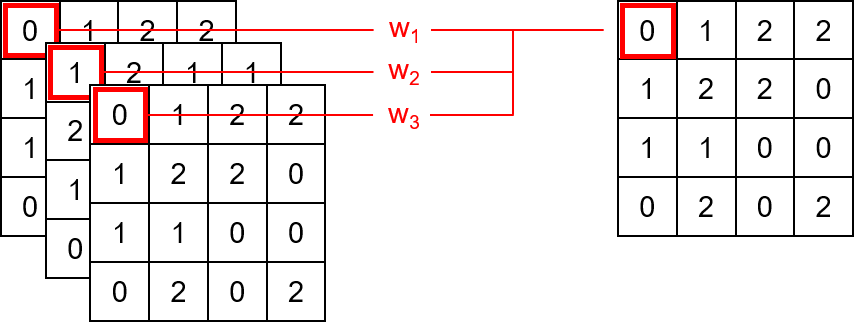
\includegraphics[width=0.8\linewidth]{img/majorityVoting2}
	\caption{Schematic representation of majority voting.}
	\label{fig:majorityVoting}
\end{figure}

\subsubsection*{Global Weighted Voting}
Global weighted voting is an atlas-based segmentation method that takes into account individual variations of the target being segmented with the available atlases. Voting of atlases with high similarity to the target being segmented are weighted higher. In our case, the T1w and T2w volumes of 20 atlases were compared with the T1w and T2w volumes of the target after a registration to an atlas volume. By measuring the mean square differences (MSD) averaged over both T1w and T2w volumes, each atlas was given a corresponding weight.  The weights were distributed by a soft maximization function so that the sum of all weights would equal one. This simplifies the calculation of the probability of the prediction. To get the segmentation, a majority voting is performed with the globally calculated weights.

\begin{figure}[h!]
	\centering
	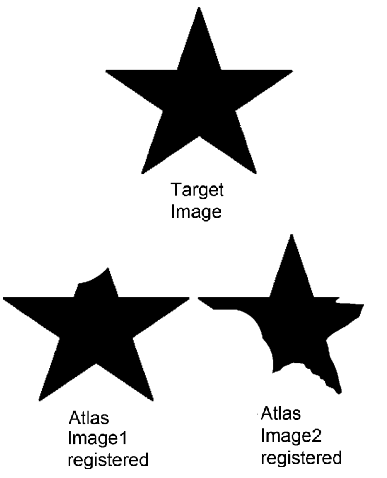
\includegraphics[width=0.5\linewidth]{img/globalWeightedProblematic}
	\caption{Example for showing the problem of global weighted voting\cite{Artaechevarria2009}.}
	\label{fig:globalweightedproblematic}
\end{figure}

The problem of this method is that an atlas is very similar in most parts but local is very different compared to the target. The weighting is still high due to the overall similarity. The opposite can also be the case, so that the overall similarity is very low but the atlas still has a very high correlation with the target in local parts. Thus, this similarity is not accounted for by the global weighting. To give this local similarities weighting, a local weighted voting can be performed. This problem is well illustrated in fig. \ref{fig:globalweightedproblematic}.

\subsubsection*{Local Weighted Voting}
The segmentation method local weighted voting takes into account local similarities of atlases with the target being segmented. Thereby, like in global weighted voting, the T1w and T2w volumes of the target and the atlases are registered to a registration atlas. Now each voxel of the atlases gets its own weighting based on the local similarity with the target. The similarities can be obtained by calculating the cross correlation, squared differences or mutual information. (see fig. \ref{fig:localWeightedVoting} for better overview) Of course, there are other similarity measures, but they have not been considered. Because the squared difference measurements give the best results for segmentation, this method was chosen\cite{b2}. Another factor is the size of the kernel which is compared locally with the target. This is not quite trivial, if the kernel is too large, a similar problem arises as with global weighted voting (see fig. \ref{fig:globalweightedproblematic}). If the kernel is too small, structures can be compared less effectively. To simplify the problem, a kernel of size 1 was chosen. Now each atlas has a whole matrix of weights instead of one similarity score, as in the global weighted voting.

\begin{figure}[h!]
	\centering
	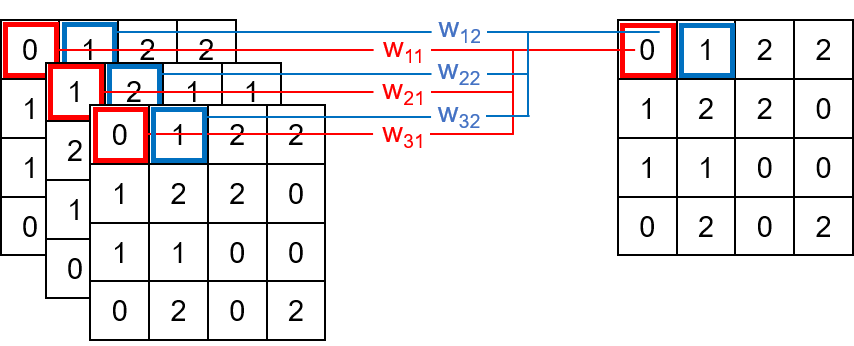
\includegraphics[width=0.8\linewidth]{img/localWeighting}
	\caption{Schematic representation of local weighted voting.}
	\label{fig:localWeightedVoting}
\end{figure}

\subsubsection*{Shape-based Averaging}
Shape-based averaging is a method introduced by \cite{Rohlfing2007}. This algorithm aims to reduce the number of unconnected region in the segmentation. Unlike the previous algorithm, this fusion method is not based on votes. The signed Euclidian distance map of each individual labels is summed up for each atlas. For each voxel, the label minimizing this sum is attributed. Formally, for $D_i$ being the signed Euclidian distance of a specific voxel $v$ for a label $l$ in the atlas $i$.
\[ l(v) = \argmin_l\sum_{i=1}^{N} D_i(v, l) \]

\begin{figure}[h!]
	\centering
	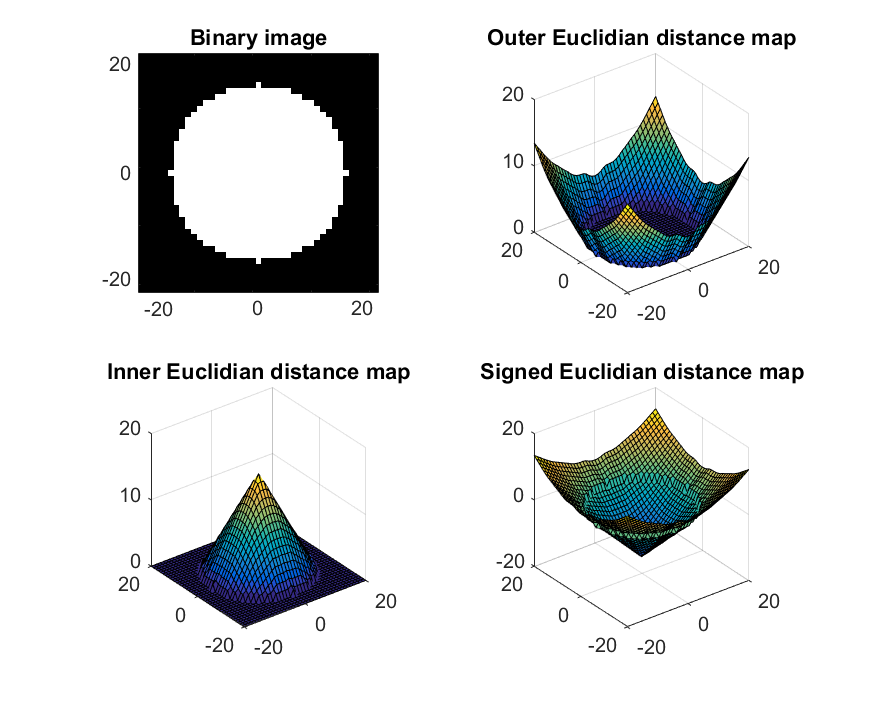
\includegraphics[width=0.8\linewidth]{img/distMap}
	\caption{Illustration of the computation steps of the signed Euclidian distance map from a simple binary image (adapted from \cite{Rohlfing2007})}
	\label{fig:distMap}
\end{figure}

\subsubsection*{Performance assessment}
This work focused on the precision aspect of the algorithm and not on the time consumption or complexity. To measure the overall performance, several evaluation metrics can be used. The Dice coefficient tells how good the computed result and the ground truth do overlap. It goes from 0 if there is no overlap at all to 1 being exactly same segmentation. The Hausdorff distance is another metric. It measures the maximum distance from the computed segmentation contour to the ground truth one. There are many more metrics that can be used to test specific characteristics of a computed segmentation. 
